\renewcommand{\theequation}{\theenumi}
\begin{enumerate}[label=\arabic*.,ref=\thesubsubsection.\theenumi]
\numberwithin{equation}{enumi}
\item In the given question,
\\
\begin{enumerate}
\item
The sample size = Total number of possibilities(S)=
$\myvec{\bmat{1&1}&\bmat{1&2}&\bmat{1&3}&\bmat{1&4}&\bmat{1&5}&\bmat{1&6}\\
\bmat{2&1}&\bmat{2&2}&\bmat{2&3}&\bmat{2&4}&\bmat{2&5}&\bmat{2&6}
\\\bmat{3&1}&\bmat{3&2}&\bmat{3&3}&\bmat{3&4}&\bmat{3&5}&\bmat{3&6}
\\\bmat{4&1}&\bmat{4&2}&\bmat{4&3}&\bmat{4&4}&\bmat{4&5}&\bmat{4&6}
\\\bmat{5&1}&\bmat{5&2}&\bmat{5&3}&\bmat{5&4}&\bmat{5&5}&\bmat{5&6}
\\\bmat{6&1}&\bmat{6&2}&\bmat{6&3}&\bmat{6&4}&\bmat{6&5}&\bmat{6&6}}$
S=6x6=36
\\
Favourable outcome for sum=2 (E1)=
$\myvec{\bmat{1&1}}$
\begin{align}
E1=1
\\
Probabilty(P(E1))=\frac{1}{36}=0.027
\end{align}
Favourable outcome for sum=3 (E2)= 
$\myvec{\bmat{1&2}&\bmat{2&1}}$
\begin{align}
E2=2 
\\
Probabilty(P(E2))=\frac{2}{36}=0.055
\end{align}
Favourable outcome for sum=4 (E3)= 
$\myvec{\bmat{1&3}&\bmat{2&2}&\bmat{3&1}}$
\begin{align}
E3=3 
\\
Probabilty(P(E3))=\frac{3}{36}=0.083
\end{align}
Favourable outcome for sum=5 (E4)= 
$\myvec{\bmat{1&4}&\bmat{2&3}&\bmat{3&2}&\bmat{4&1}}$
\begin{align}
E4=4
\\
Probabilty(P(E4))=\frac{4}{36}=0.111
\end{align}
Favourable outcome for sum=6 (E5)= 
$\myvec{\bmat{1&5}&\bmat{2&4}&\bmat{3&3}&\bmat{4&2}&\bmat{5&1}}$
\begin{align}
E5=5
\\
Probabilty(P(E5))=\frac{5}{36}=0.138
\end{align}
Favourable outcome for sum=7 (E6)= 
$\myvec{\bmat{1&6}&\bmat{2&5}&\bmat{3&4}&\bmat{4&3}&\bmat{5&2}&\bmat{6&1}}$
\begin{align}
E6=6
\\
Probabilty(P(E6))=\frac{6}{36}=0.166
\end{align}
Favourable outcome for sum=8 (E7)= 
$\myvec{\bmat{2&6}&\bmat{3&5}&\bmat{4&4}&\bmat{5&3}&\bmat{6&2}}$
\begin{align}
E7=5
\\
Probabilty(P(E7))=\frac{5}{36}=0.138
\end{align}
Favourable outcome for sum=9 (E8)= 
$\myvec{\bmat{3&6}&\bmat{4&5}&\bmat{5&4}&\bmat{6&3}}$
\begin{align}
E8=4
\\
Probabilty(P(E8))=\frac{4}{36}=0.111
\end{align}
Favourable outcome for sum=10 (E9)= 
$\myvec{\bmat{4&6}&\bmat{5&5}&\bmat{6&4}}$
\begin{align}
E9=3 
\\
Probabilty(P(E9))=\frac{3}{36}=0.083
\end{align}
Favourable outcome for sum=3=11 (E10)= 
$\myvec{\bmat{5&6}&\bmat{6&5}}$
\begin{align}
E10=2
\\
Probabilty(P(E10))=\frac{2}{36}=0.055
\end{align}
Favourable outcome for sum=12 (E11)=
$\myvec{\bmat{6&6}}$
\begin{align}
E11=1
\\
Probabilty(P(E11))=\frac{1}{36}=0.027
\end{align}
Table is completed as follows:
\resizebox{\columnwidth}{!}{%
\begin{tabular}{|c|c|c|c|c|c|c|c|c|c|c|c|}
\hline
Event:'Sum on two dice'&2&3&4&5&6&7&8&9&10&11&12\\
\hline
Probability&$\frac{1}{36}$ &$\frac{2}{36}$&$\frac{3}{36}$&$\frac{4}{36}$&$\frac{5}{36}$&$\frac{6}{36}$& $\frac{5}{36}$ &$\frac{4}{36}$&$\frac{3}{36}$&$\frac{2}{36}$& $\frac{1}{36}$\\
\hline
\end{tabular}
\label{table:1}
}
\end{enumerate}
\begin{enumerate}
\item The argument mentioned by the student is incorrect.
\\
In the question the event of measurement is sum of possible outcomes of rolling two dice.
Here, the probability of occurence of each outcome is not equal. 
\\
The different values of probabilities are mentioned in the above solution.
\\
The argument can be supported by the figure \ref{fig:figure1}
\\ 
The python code for the figure \ref{fig:figure1}
\begin{lstlisting}
prob/codes/prob3.py
\end{lstlisting}
shows the random distribution of data.
\begin{figure}[!ht]
\centering
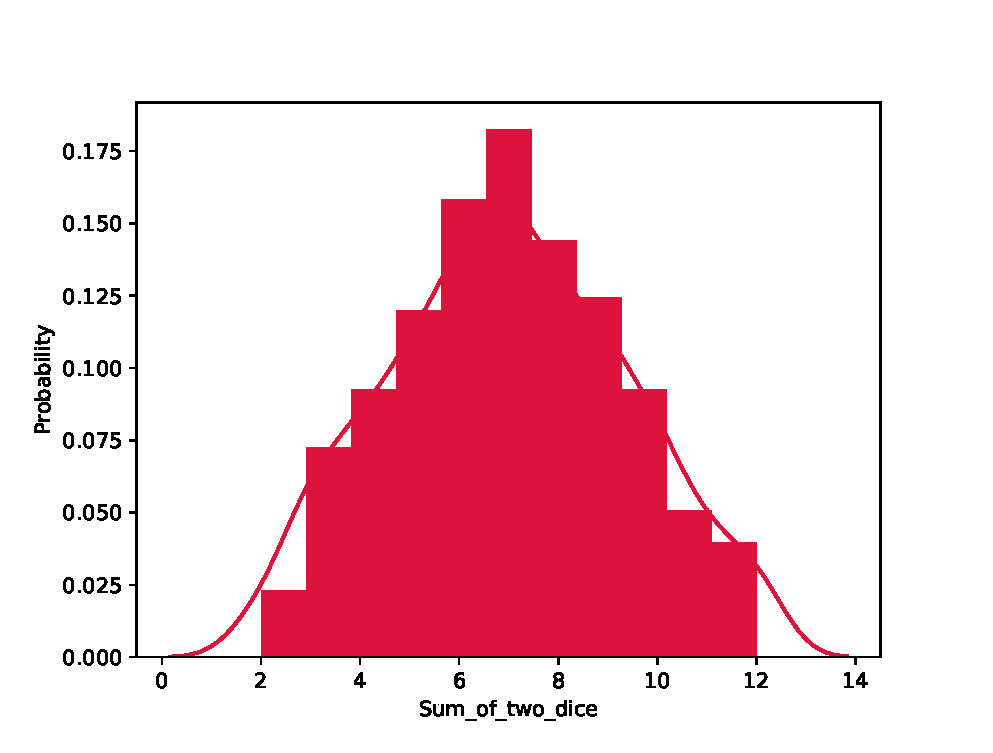
\includegraphics[width=\columnwidth]{./prob/figs/prob3.eps}
\caption{}
\label{fig:figure1}
\end{figure}
The Distribution of data is given below
\\
Probability mass function(P(X=k))=
\begin{align}
\bmat{\frac{k-1}{36}& for x<8\\\frac{13-k}{36}& for x=>8}
\end{align}
The understanding of the curves \ref{fig:figure1} can be seen in \eqref{understandingcurve}
\end{enumerate}
\end{enumerate}